\documentclass[12pt]{report}

\usepackage[utf8]{inputenc}
\usepackage{amsmath}
\usepackage{amsfonts}
\usepackage{amssymb}

% Line spacing
\usepackage{setspace}
%\onehalfspacing
\doublespacing

% Figures
\usepackage{caption}
\usepackage{graphicx}
\usepackage{hyperref}
\usepackage{multirow}

% Matrix packages
\usepackage{blkarray}
\usepackage{amsmath}


% Margin adustment
\addtolength{\oddsidemargin}{-.875in}
\addtolength{\evensidemargin}{-.875in}
\addtolength{\textwidth}{1.75in}
\addtolength{\topmargin}{-.875in}
\addtolength{\textheight}{1.75in}

% Paragraph indentation
\usepackage{changepage}

\author{Lillian Tatka}
\title{In Silico Evolution of Oscillating Mass-Action Chemical Reaction Networks}
\begin{document}
\begin{titlepage}
\begin{center}

%\begin{spacing}{1.5}
%Internship Project Report\\
%\vspace*{\fill}
%\end{spacing}
\begin{spacing}{2.5}
In Silico Evolution of Oscillating Mass-Action Chemical Reaction Networks
\vspace*{\fill}
%\textit{Submitted by}
\end{spacing}

\begin{spacing}{1.15}
Lillian Tatka

\vspace*{\fill}


A dissertation\\submitted in partial fulfillment of the\\requirements for the degree of
\\
\vspace*{\fill}
Doctor of Philosophy\\
\vspace*{\fill}
University of Washington\\
2024
\vspace{\fill}

Reading Committee:\\
Herbert Sauro, Chair\\
Patrick Boyle\\
Lucian Smith\\


\vspace*{\fill}
Program Authorized to Offer Degree:\\
Bioengineering

\end{spacing}
\end{center}
\end{titlepage}

%\maketitle
\null
\begin{center}
\textcopyright Copyright 2024\\
Lillian Tatka
\end{center}
\pagenumbering{gobble}
\newpage

\pagenumbering{roman}
\begin{center}
University of Washington\\
\vspace*{\fill}
\textbf{Abstract} \\
\vspace*{\fill}
In Silico Evolution of Oscillating Mass-Action Chemical Reaction Networks\\
\vspace*{\fill}
Lillian Tatka\\
\vspace*{\fill}
Chair of the Supervisory Committee:\\
Herbert Sauro\\
Bioengineering
\pagenumbering{gobble}
\end{center}
\vspace*{\fill}
Computational models are increasingly used in high-impact decision making in science, engineering, and medicine. It is crucial that computational models meet a standard of credibility when using them in high-stakes decision making. For this reason, institutes including NASA, the FDA, and the EMA have developed standards to promote and assess the credibility of computational models and simulations. However, due to the breadth of models these institutes assess, these credibility standards are mostly qualitative and avoid making specific recommendations. On the other hand, modeling and simulation in systems biology is a narrower domain and several standards are already in place. These factors facilitate the development of a quantitative credibility standard. A systems biology credibility standard is essential given the rise in complexity and influence of models. This proposal describes the development of a testing suite to standardize and automate credibility testing and scoring of computational systems biology models. The test suite will include dynamic tests that examine the output of a simulated model, verification and validation tests, and a preliminary assessment of parameter sensitivity to gauge uncertainty in the model's predictions. 

\tableofcontents



\chapter{Introduction}
\pagenumbering{arabic}
The \textit{in silico} evolution of chemical reaction networks can be a useful tool to create functional networks with specific behaviors as well as to investigate possible pathways of natural evolution. Large sets of synthetic networks can be useful for exploring design patterns and network motifs, gathering statistics network characteristics, benchmarking software, and informing design of synthetic networks. Although several studies use \textit{in silico} evolution to generate networks, the vast majority of them focus on genetic regulatory networks, and almost none of them provide software for others to reproduce their results or use evolutionary strategies in other work. A fast and user-friendly software package would allow researchers to experiment with \textit{in silico} evolution without significant knowledge of programming. 

The key objective of this work is to produce a software package that enables the \textit{in silico} evolution of mass-action chemical reaction networks and to explore features and hyperparameters of the evolutionary algorithm that influence the evolution of oscillatory reaction network. The software should be accessible to researchers with minimal programming experience, produce results relatively quickly, and be problem agnostic, meaning that a variety of behaviors could be evolved.  

This project began with the creation of a python tool to evolve oscillating chemical reaction networks. Described in chapter \ref{chap: cesium_paper}, this work was intended as a small initial step towards understanding the function of biochemical oscillators and identifying common design patterns that enable oscillation. Oscillating systems of are of particular interest due to their biological relevance and interesting dynamics and serve as a good candidate problem due to the presence of an intermediate state (damped oscillations). A large population of oscillators was computationally evolved and their reaction characteristics compared to non-oscillating systems. The library of reaction networks generated in this research was used to construct a publicly available database to enable further oscillator/design pattern research as well as to serve as a standardized data set for testing novel software and algorithms. 

However, the algorithm used to generate these oscillating networks had its flaws. It took a long time to execute, several minutes per run, and failed to generate oscillators most of the time. Only approximately 5\% of evolution trials would result in an oscillator. It took several days of computing time to generate the small database. The most likely cause of this low success rate was the rapid convergence of solutions. The design of the algorithm allowed the most fit reaction networks to dominate the population, even if they were not oscillators or close to becoming oscillators. This dominance would reduce the space for innovation and prevent more fit networks from developing. If a promising candidate network failed to develop in the first few generations, it was unlikely that the evolution trial would be successful.

Additionally, the structure of the code and algorithm did not allow for easy modification and exploration. For example, a user might wish to implement a different selection technique in an attempt to avoid the problem of rapid convergence, but the software was not created to allow for such tinkering. Users could modify some hyperparameters, such as the number of generations and population size, but the fundamental evolution algorithm could not be modified. 

To address these shortcomings and explore evolution strategies for mass-action reaction networks, a new software tool was developed, NetEvolve, described in detail in chapter \ref{chap: NetEvolve}. The software is written in the Julia programming language [CITTEEEEE], which uses just-in-time (JIT) compiling, type stability, and multiple dispatch to gain significant speed advantages over interpreted languages such as Python. The evolution algorithm can be used immediately using default settings or customized using a JSON file. By default, the algorithm evolves oscillators, but users could provide any time series data and the algorithm would attempt to generate networks to match. 

To combat premature convergence, NetEvolve separates candidate reaction networks into groups based on similarity. These groups are analogous to species in natural evolution and individuals are compared only against members of the same species. This prevents more fit candidate networks from dominating the population and shelters network innovations that may reduce fitness at first but develop into useful features over the course of several generations. 

Inspired by the use of evolutionary algorithms to create artificial neural networks, NetEvolve also implements a form of crossover, a mutation operator that combines features from two ``parent" networks to create a new ``offspring" network. This feature was shown to improve evolution performance when evolving artificial neural networks and genetic regulatory networks, but has been thought to be disruptive for evolving mass-action networks. The application of crossover to mass-action networks is explored in detail in chapter \ref{chap: NetEvolve}.

\begin{itemize}
\item\textbf{Aim 1:} Develop a python package to perform dynamic tests on systems biology models in order to assess their credibility
\item\textbf{Aim 2:} Create tools to automatically verify and validate models
\item\textbf{Aim 3:} Build software to automate simple parameter sensitivity analyses
\end{itemize}

This research will result in two first author publications, the titles of which are to be determined. The first publication will describe the design and purpose of the software package and include some preliminary examples of implementation. The second publication will present the full software package and demonstrate its use on several existing models. I hope to finish this work by June 2024.

\section{A brief history of chemical oscillators}
The first oscillating chemical system was described in 1828. Gustav Fechner described and electrochemical cell that produced an oscillating current. Later, in 1899, Fredriech Ostwald observed that the rate of chromium dissolution in acid periodically increased and decreased. Both these systems were heterogenous mixtures, leading to the belief that homogenous oscillating reactions were impossible, a belief that persisted through much of the 20th century. Their relatively recent discovery and study makes homogenous chemical oscillators a topic of particular interest. Mentions of "oscillators" in this dissertation refer to this type of chemical oscillator.

Prior to leaving science to work for an insurance company, Alfred Lotka authored a monograph on theoretical biology. In 1910, he showed that a set of consecutive mass-action reactions can create damped oscillators which eventually settle at an equilibrium. A decade later he published a second paper on mass-action oscillatory systems. ALthough this publication did not apply to any real chemical system, it's dynamics inspired Vito Volterra to apply the model to ecology. The Volterra used similar ideas to investigate migration effects and interactions between several species. The Lotka-Volterra model is well-known today as a simple representation of predator-prey interactions, where both populations oscillate in time.

The Lotka-Volterra model consists of three irreversible steps describing the relationships between grass, rabbits, and lynxes. A represents grass, which is assumed to be constant. Rabbits, represented by X, consume grass to grow their population (equation \ref{eqn: LV_1}). Lynx, in turn, consume rabbits to grow their population (equation \ref{eqn: LV_2}) before eventually dying (equation \ref{eqn: LV_3}).

\begin{equation}
\label{eqn: LV_1}
A + X \to 2X
\end{equation}
\begin{equation}
\label{eqn: LV_2}
X + Y \to 2Y
\end{equation}
\begin{equation}
\label{eqn: LV_3}
Y \to P
\end{equation}

These ``reactions" assume ``mass-action" kinetics where the rate of each depends on the amount of grass (constant) and sizes of the population of rabbits and lynx respectively. These rates can be described by the following differential equations, where ${k_{y}}$ describes the rate of lynx reproduction given a rabbit of population size ${x}$, ${k_{d}}$ describes the mortality rate of lynx, and ${k_{x}}$ describes the rate at which rabbits reproduce. The population of rabbits and lynxes will oscillate for any set of these constants.

\begin{equation}
dx/dt = k_{x}ax - k_{y}xy
\end{equation}
\begin{equation}
dy/dt = k_{y}xy - k_{d}y
\end{equation}

The oscillations in this system result from the time delay between the growth in rabbit population growth and lynx population growth as well as the delay from rabbit population decline to lynx decline. Rabbits reproduce because grass is in constant supply. As the rabbit population grows, the lynx population follows as prey becomes plentiful. Once the lynx population gets too high, it will begin consuming rabbits at a rate faster than they can reproduce due to the constant supply of grass. Once the rabbit population declines, the lynx population will follow as food grows scarce and they begin to starve. When the lynx population is depleted, there will be less predation pressure and the population of rabbits will begin to grow again. This phenomenom can be observed in nature. Figure XXXX shows the oscillating populations of Canada lynx and Snowshoe hares from 1850 to 1920. The predator-prey model has also been demonstrated in the laboratory with paramecia that eat yeast (FIGURE XXX AND CITATION).

A key feature of this oscillating system, and of most chemical oscillating systems is the presence of autocatalysis. The rate of growth of a population increases as the size of the population increases. The prominence of autocatalysis is also observed in the evolution of \textit{in silico} theoretical chemical reaction networks, as is described in chapter \ref{chap: cesium_paper} and the associated publication [CITATION]. In chemical systems, autocatalysis serves as a from of positive feedback to drive oscillation.

[MORE STUFF HERE ABOUT AUTOCATALYSIS- POSITIVE FEEDBACK in oscillators]

From Kumar and Sharma 2006

Even though oscillators might appear to violate second law of thermodynamics, they down because it is driven by decrease of Gibbs-free energy of an overall chemical reaction occurring far from thermo equilirbium.  These are thermodynamically open systems.

Long lasting oscillations occur only if the proper feedback mechanism is present.
Presence of 1+ autocatalyic step leads to oscillations, but you can get an explosion as product concentration keeps building, so you need an inhibition step too. But if these occur at the same time, you stabilize the steady state and don't get oscillations, so the inhibition step has to be delayed.

You need bistability (?). and some intermediate that reacts with both X and Y which allows the system to periodically switch between the steady states.

Tyson Book section
2 component oscillators: need autocatal and negative feedback. 

At some point might want to mention this paper; "Evolution of Autocatalytic Sets in Computational Models
of Chemical Reaction Networks"

"""
Most oscillators are associated with unstable steady states. Destabilizing processes can be classified as 1) direct autocatalysis, 2) indirect autocatalysis (a positive feedback loop), and 3) end-product inhibition (a negative feedback loop)~\cite{Tyson1975, tyson2007}. Reactions are considered autocatalytic when the products increase the rate of reaction or when a chemical decelerates the rate of its own destruction~\cite{Tyson2004}. Given the two types of oscillators, negative feedback and negative feedback coupled with positive feedback~\cite{Sauro_dynamics}, it is unsurprising that autocatalytic reactions are enriched in the oscillator population as these reactions are a form of positive feedback."""

\chapter{A Public Database of Evolved Oscillatory Reaction Networks}
\label{chap: cesium_paper}
\section{Background}
With the constant emergence of new software tools and techniques in systems biology, access to a large variety of chemical reaction network models with defined characteristics can be useful for testing and validation. For example, an existing data set enumerating small chemical reaction networks~\cite{deckard2009} has been used to test computational methods to analyze bistability~\cite{pantea2010}, software to reverse engineer networks~\cite{nobile2013}, and a novel framework to assess networks for multiple equilibria and other characteristics~\cite{donnell2014}. Generating these test data sets can be computationally expensive and time-consuming. The data set generated by Deckard et al. took several days to compute and contains approximately 47 million small models, but its purpose is to exhaustively enumerate small networks, not to assess and catalog their behavior~\cite{deckard2009}.  Despite the usefulness of standard validation data sets, currently no public database exists containing numerous models displaying a variety of network behaviors.

In terms of network behavior, oscillatory chemical reaction networks are of particular interest due to their biological relevance, including embryogensis, DNA repair, and heart function~\cite{Novak2008,Aulehla2008,GevaZatorsky2006, Pol1928}. Lotka et al. documented the first ordinary differential equation model of an oscillatory predator-prey network~\cite{Lotka1910}. The study of oscillatory mechanisms in chemical reaction networks dramatically increased with the expansion of computing power and the improved ability to solve non-linear differential equations~\cite{Higgins1967}. Novak and Tyson studied non-autocatalyic small oscillators to determine design patterns and basic requirements for oscillating systems~\cite{Novak2008}. These works focus on the mechanisms and characteristics of individual oscillators or to oscillators as a broad category. Paladugu et al. used in silico evolution to create several oscillators, bistable switches, homeostatic systems and frequency filters, but the library was not made publicly available for further study~\cite{Paladugu2006}. 

We present a public database, entitled "Cesium",  containing approximately 1800 3-species, 450 6-species, and 750 10-species oscillating networks created using a customized evolution algorithm, an optimization process based on the iterative improvement of candidate models. There are also random non-oscillating networks to serve as controls. The database can be searched by the number of reactions, the presence of autocatalytic reactions, and the number of species. Each entry contains the above information as well as the Antimony string~\cite{Smith2009} of the model which can be simulated by any software capable of reading antimony or SBML (to which Antimony models can be converted). Future work will expand this database to include a wider variety of oscillatory models as well as models that display other behaviors such as bistability. 

The population of evolved oscillatory reaction networks possessed different reaction type compositions compared to non-oscillating networks that were randomly generated. Oscillating networks had significantly more uni-bi reactions and autocatalytic reactions. 


The purpose of this research is two-fold: basic research into characteristics of oscillatory systems, and the development of this database.

The availability of a standardized database for use in software and algorithm testing pushed me in the direction of model credibility. This is a step beyond reproducibility, the goal of which is the easy reproduction of a model and its results by third party users. Credibility refers to the trustworthiness of a model. This topic and related research will be covered in later chapters.

\section{Methods}



Oscillating models were generated using evolution scripts written in python, available at https://github.com/sys-bio/evolution. The process begins by randomly generating a population of models and gradually modifying them over time to produce oscillatory behavior. Four types of reactions are used: uni-uni, uni-bi, bi-uni, and bi-bi, all with mass-action kinetics (figure \ref{fig:reaction}). At each step, every model is evaluated against an objective function scoring the model's ability to oscillate. Models with better fits are selected and further modified and models with lower fits are gradually eliminated. 
% \begin{wrapfigure}{r}{0.5\linewidth}
% \centering
\begin{figure}
    \centering
    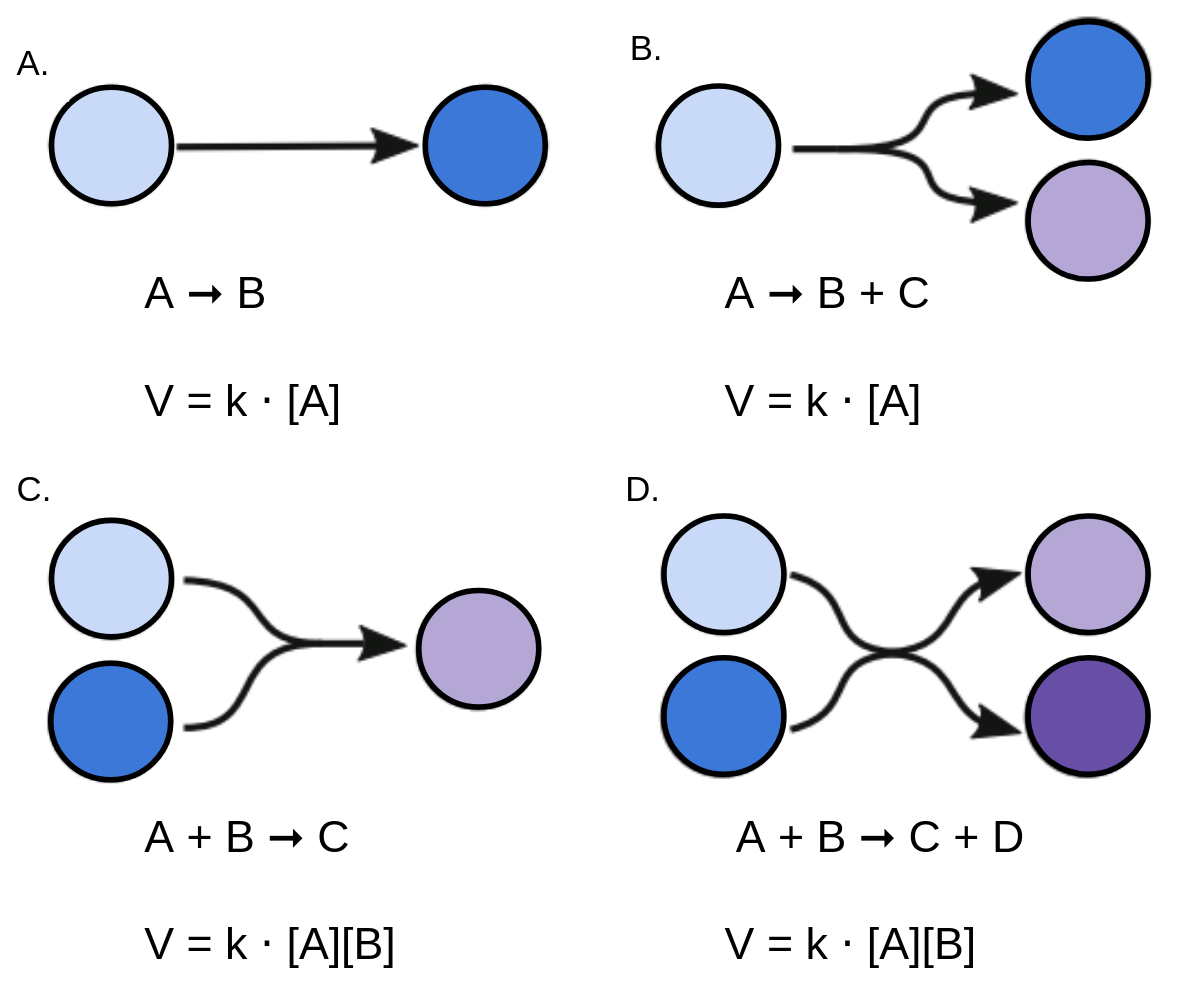
\includegraphics[width=7cm]{images/Reactions.png}
    \captionof{figure}{Models were composed of four reaction types and rate laws: (A) uni-uni, (B) uni-bi, (C) bi-uni, (D) bi-bi}
    \label{fig:reaction}
    
\end{figure}





\subsection{Model Representation}

Models and reactions were represented by custom data structures. An instance of the \textit{reaction} object represents a single reaction and consists of one or two reactants, one or two products, a rate constant, and an integer representing the reaction type (uni-uni, uni-bi, bi-uni, or bi-bi). The \textit{model} object represents a single reaction network and consists of a list of species, a list of initial concentrations, and a list of \textit{reaction} objects. The software converts \textit{model} objects into systems of ordinary differential equations which are then numerically solved to produce time series data of species concentrations. After the evolution process is complete, the models are converted to antimony~\cite{Smith2009}, a human readable model definition language.

\subsection{Objective Function}

The objective function minimized error between the candidate model's time course data and a series of points corresponding to the peaks and troughs of an oscillator. This "idealized" oscillator time series consisted of nine concentration points, alternating between 5 and 30 concentration units over the course of 1.25 seconds (figure \ref{fig:fitness}). The output time series of each species was compared to these points by summing the squared difference between the observed point and the ``ideal" point and the smallest error value was considered the model's fitness. This is similar to MSE but the sum is not divided by the number of observations as this number is constant across all models. This has been demonstrated to be an effective objective function for the in silico evolution of chemical oscillators~\cite{Paladugu2006}.  In cases where candidate models could not be simulated, an arbitrarily high fitness value was assigned resulting in their subsequent removal from the population in the selection step.  

\begin{figure}
    \centering
    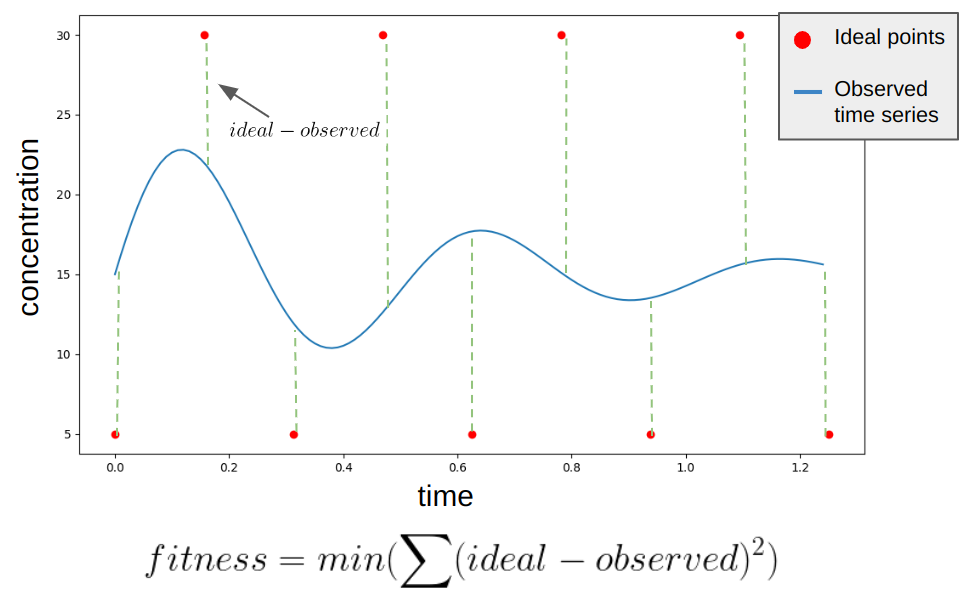
\includegraphics[width=10cm]{images/fitness.png}
    \captionof{figure}{For the time series data of this species, the error is calculated by summing the square difference between the observed time series data (blue) and a set of idealized oscillator points (red). This process is repeated for each species in the model and the fitness is defined as the minimum of these sums. }
    \label{fig:fitness}
\end{figure}

\subsection{ODE Solver}
Preliminary studies suggested that the most commonly used python ODE solver from scikit was inaccurate for solving these problems. Other off-the-shelf solvers lacked the ability to deal with the custom data structure encoding the models. The Sauro Lab's simulation software, RoadRunner~\cite{Somogyi2015}, was also unsuitable for this purpose due to the computational cost of frequently modifying and recompiling models for simulation. Many algorithms, such as RK4 are not robust enough for this work. For this reason, a custom simulator using the CVODE solver from the Sundials suite was used~\cite{hindmarsh2005sundials}. 

\subsection{Selection}
In each new generation, the top 10\% of models from the previous generation were copied without modification. The remainder of the new population was chosen by tournament selection~\cite{Miller1995} from the previous generation. This is where two models are randomly chosen from the previous generation (including from the top 10\% of models already carried over) and the model with the better fitness is mutated by adding or deleting a reaction, or by modifying a rate constant. The modified model is then appended to the new generation. 

\subsection{Mutation}
After tournament selection, the fitter model was either mutated by modifying a rate constant or adding/deleting a reaction with equal probability. In the case of rate constant modification, a random rate constant was adjusted by a random percentage between -15\% and +15\% of the rate constant's current value. This mechanism ensured that rate constants could not become negative, and there was no upper limit to their value. 

In the case of reaction modification, a reaction was either added or deleted with 50\%-50\% probability. If deleted was selected, a random reaction was removed from the model. If addition, a new reaction was added with the equal probability of each reaction type: uni-uni, uni-bi, bi-uni, bi-bi (figure~\ref{fig:reaction}). 

\subsection{Random Networks for Evolution}
A population of 40 random networks were generated using the {\tt teUtils} python package~\cite{SauroteUtils_2020}. Each network was initialized with three species, and nine reactions with the probability of each reaction type being 0.1, 0.4, 0.4, 0.1 for uni-uni, uni-bi, bi-uni, and bi-bi reactions. These settings were chosen to maximize the number of evolution trials that successfully product oscillators. All reactions had mass-action kinetics with a random rate constant between 0 and 50. 
\begin{figure}
    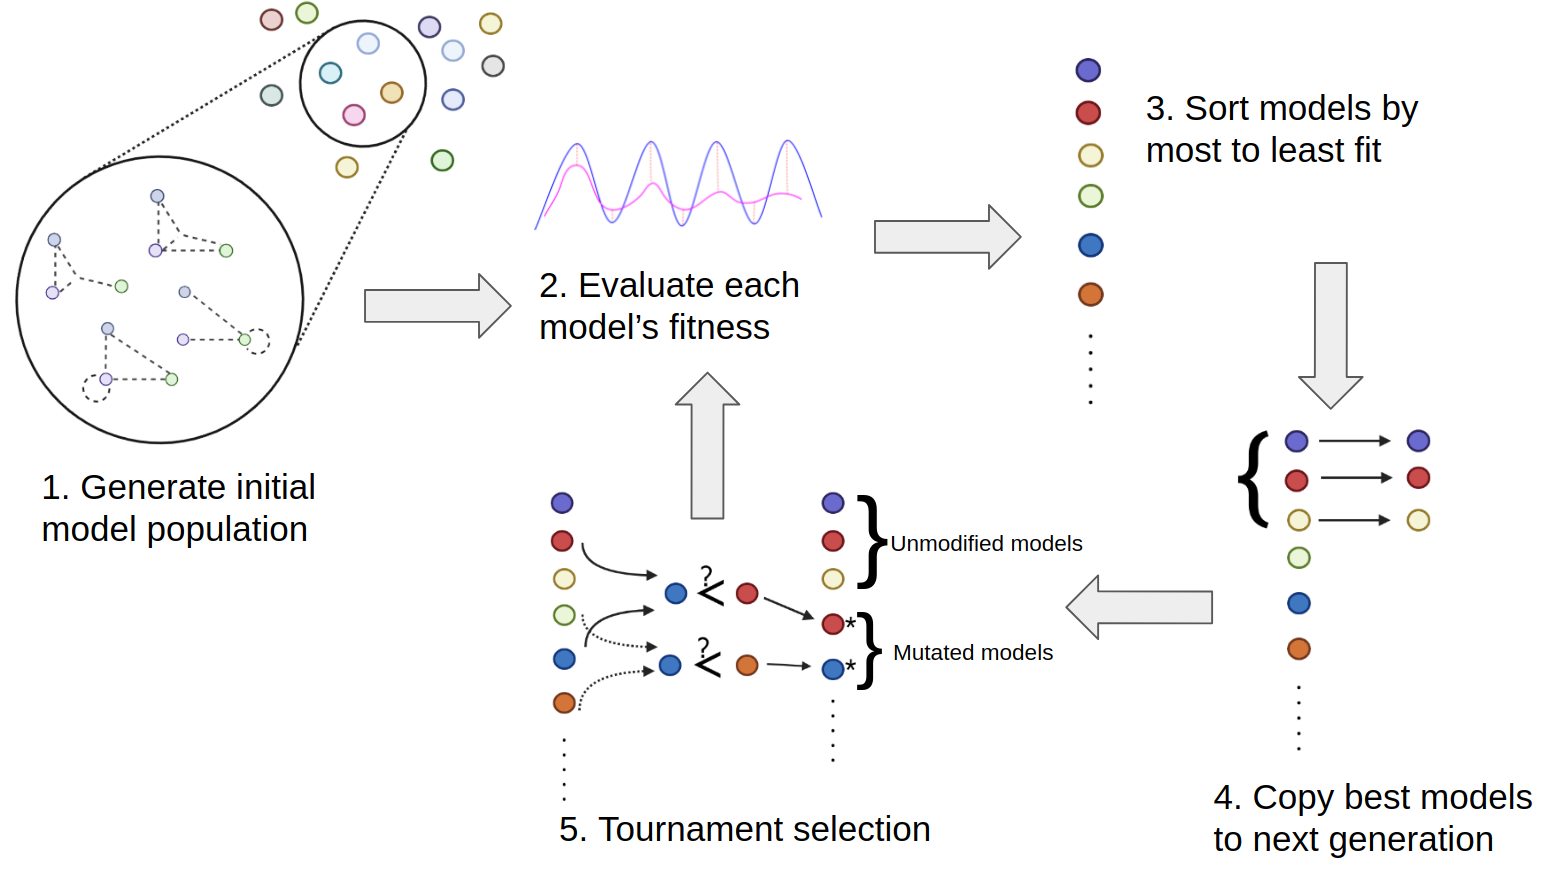
\includegraphics[width=12cm]{images/algorithm.png}
    \captionof{figure}{The evolution algorithm. (1) An initial population of random models is created. (2) The fitness of each model is evaluated. (3) The entire population is sorted by most fit to least fit. (4) The top 10\% of the models are transferred to the subsequent generation unmodified. (5)  Tournament selection is used to populate the remainder of the subsequent generation. Models are randomly selected, the more fit model is chosen to be modified and carried over to the subsequent generation. Steps 2-5 are repeated. }
    \label{fig:algorithm}
\end{figure}

\subsection{Custom Evolution Algorithm}

The evolutionary algorithm mimics biological evolution in that populations of individuals, in this case candidate networks, are altered and forced to compete with each other. Over the course of generations, fitter individuals (models that oscillate or are likely to oscillate) out compete unfit individuals (models that do not oscillate or can not be simulated) and survive into the next generation. Although genetic and evolutionary algorithms are well characterized, their application to systems biology models remains a challenge as a key trait in these algorithms is crossover, the ability of two possible solutions to exchange information, creating a new, ideally more suitable, candidate solution~\cite{Katoch2020}. Typically, genetic algorithms operate on objective functions for which solutions consist of vectors where values can easily be exchanged between two vectors. It is uncertain how crossover of mass-action kinetic models could be achieved as solutions (candidate networks) consist both of topology (how reactions are connected) as well as rate constants (vectors of values). Additionally, the number of reactions and rate constants vary and must be equal but can vary from model to model. For this reason, a custom optimization process was developed based on genetic algorithms but avoiding crossover. 

This process begins with the generation of 40 random networks with pre-specified probabilities for each of the four reaction types.  The fitness of each model is evaluated by comparing the model's time series data with an objective function representing the desired outcome, oscillation. Models that with time series data close to this desired outcome, those that oscillate or those with damped oscillations, are more fit than those that fail to oscillate or cannot be simulated. 

These models are ordered from most to least fit and the top 10\% of the models are carried over unmodified to the subsequent generation (figure \ref{fig:algorithm}). The remaining models are randomly paired and compared and the fitter of the two models is slightly modified by either adding or deleting a reaction or changing a rate constant. If the modification improves the fitness of the model, the modified model is added to the next generation. If the modification makes the model less fit, 75\% of the time the unmodified model is added to the next generation and 25\% of the time the less fit model will be added. This allows for the chance that small changes initially make a model worse, but subsequent changes drastically improve the model. Once the new generation is fully populated, the models are again ordered from most to least fit and the process begins again. This is repeated for 400 generations or until a threshold fitness level is reached.

\subsection{Random Control Networks}
Random models were generated as described in the previous section. To control for changes made during evolution, the random models underwent the same mutation processes described previously. Instead of populating subsequent generations based on model fitness, 10\% of the previous population was randomly selected to be carried over unmodified to the new generation. The remainder of the new generation was populated with models randomly chosen and mutated from the previous generation. The purpose of this procedure was to account for model variability introduced in the evolutionary process. Of 1000 random control networks generated, 1 was a spontaneous oscillator.

\section{Results}
Evolved models are processed to remove any undesirable oscillators from the population, namely oscillators that dampen over time or oscillators where one or more species concentrations rise indefinitely towards infinity. Next,  duplicated reactions were fused and reactions that are superfluous to oscillation are deleted to minimize network size resulting in a population of reaction networks that oscillate indefinitely in species concentration, examples of which are shown in figure 4.

\begin{center}
    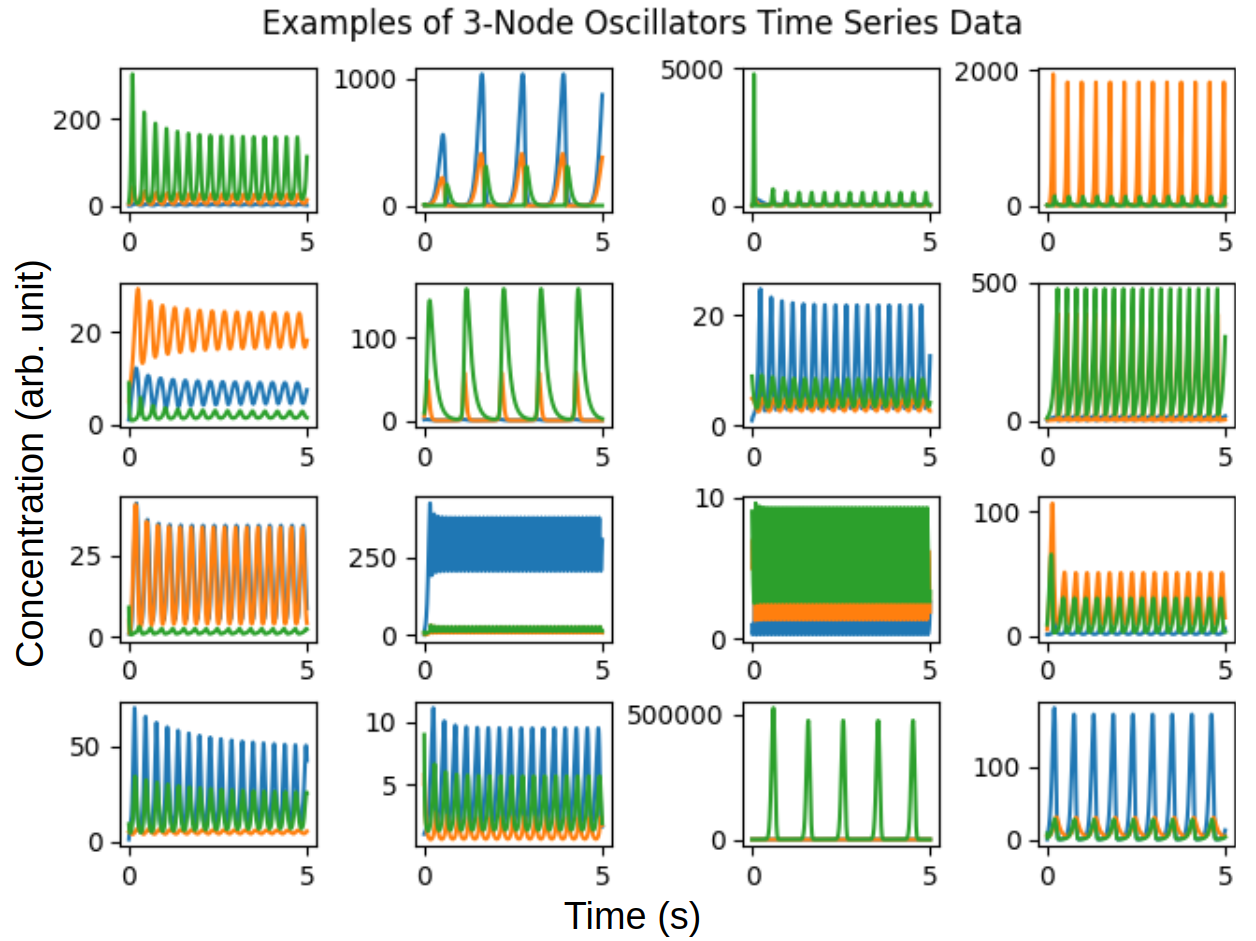
\includegraphics[width=8.5cm]{images/examples.png}
    \label{fig:examples}
    \captionof{figure}{Time series data of sixteen 3-node oscillators generated using differential evolution.}
\end{center}


\subsection{Database Construction}
A non-relational key-value database was deployed via Mongo Atlas using the PyMongo API to store all models and their information. The user enters the desired reaction network attributes into the web GUI (figure \ref{fig:website}). Models are downloaded as a .zip file of text files, or if a single model a single text file, containing the antimony string of each model. If the "Download in simulatable Tellurium form" box is checked, then each model file will contain the necessary python package imports and formatting to be immediately simulated and plotted upon running the file.


The current website queries the database by model type (current options are oscillator or random), the number of nodes (species), the number of reactions, and the presence or absence of autocatalysis or degradation reactions. Both oscillator and non-oscillating control networks are stored in the database. Each entry also includes a dictionary of tallies of each reaction type in the network, a list of redundant reactions that were fused during post-processing, a list of reactions that were deleted as their presence did not influence oscillation. 




In addition to the Antimony string comprising the model, other characteristics such as its initial reaction probabilities, fused and deleted reactions, and reaction counts are also tracked in the database.  The database can be queried to select models with any number of desired traits. Both oscillator and non-oscillating control networks are stored in the database.

The Cesium database is publicly available on the web at \url{https://cesiumdb.herokuapp.com/} and is intended to serve as source of reaction networks with specified characteristics for use in research and validation.  It currently contains 2000 randomly generated models and approximately 1800 3-species oscillating networks. This database can be expanded in the future to include a wider variety of oscillatory networks as well as networks with different behaviors, such as bistability. 

\begin{figure}
    \centering
    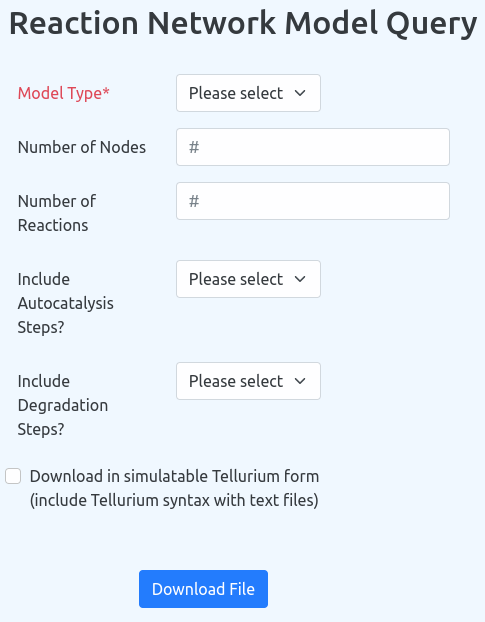
\includegraphics[width=8cm]{images/website.png}
    \captionof{figure}{Landing page for the Cesium database.}
    \label{fig:website}
\end{figure}

\subsection{Oscillating Network Examples}
Four oscillating networks from the database are shown in figure \ref{fig:model-diagrams}. Arrows symbolize reaction and lead from the reactant to the product. A double headed arrow indicates two products are formed and a double tail indicates two reactants. 


\begin{figure}
    \centering
    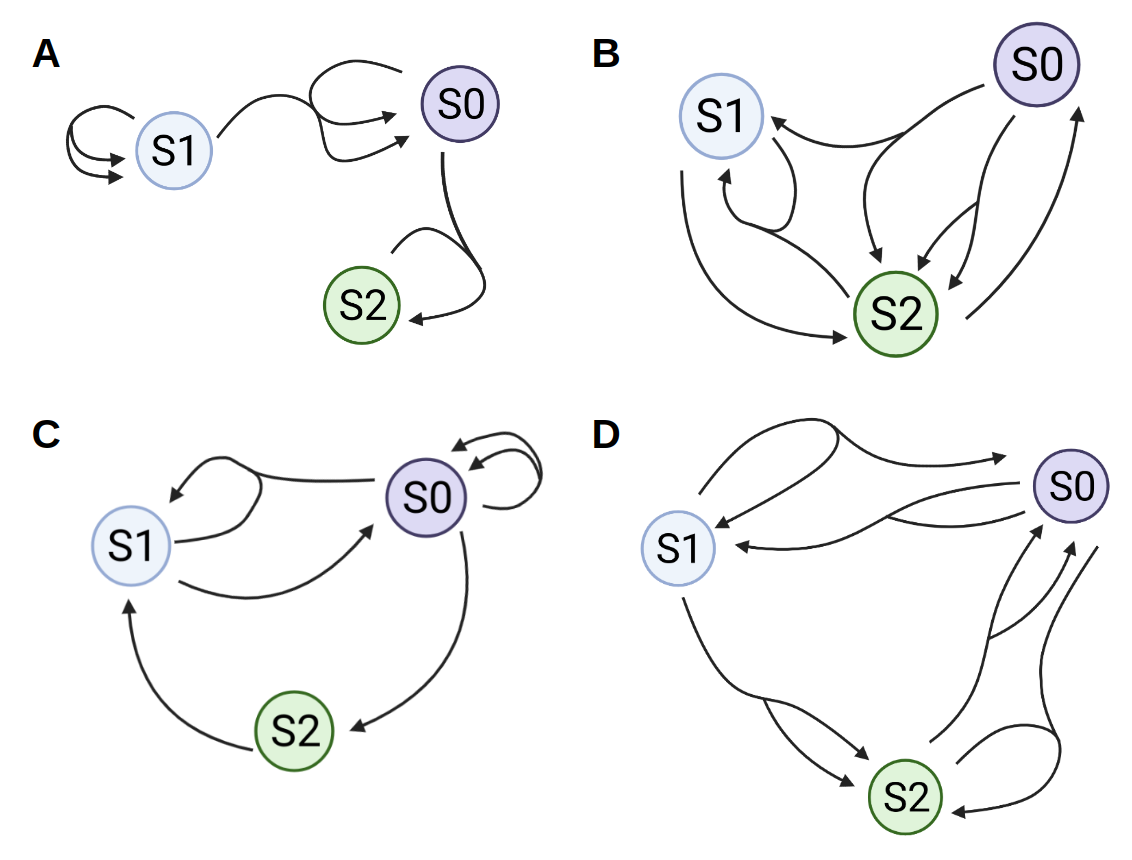
\includegraphics[width=8cm]{images/model-diagrams.png}
    \captionof{figure}{Examples of 3-species oscillating networks from the Cesium database.}
    \label{fig:model-diagrams}
\end{figure}

In network A, S1 is autocatalytic as is S0 (and catalyzed by S1). These linked positive feedback loops cause oscillation with products out flowing to S2, which essentially behaves as a boundary species, a species that is unaffected by the model and whose concentration remains fixed.  Network B lacks autocatalytic reactions completely. Computing the jacobian matrix at the unstable focus results in the following matrix:
\[
\begin{blockarray}{cccc}
S0 & S1 & S2 \\
\begin{block}{(ccc)c}
  -4.75 & 0 & 15.2 & S0 \\
  0.75 & -0.3 & 0 & S1 \\
  8.75 & -1.6 & -22.8 & S2 \\
\end{block}
\end{blockarray}
 \]
In the bottom row center, the negative number indicates that there is an inhibitory relationship between S1 and S2. An increase in S2 will decrease the production rate of S1. These interactions for a cycle with negative feedback, suggesting that this is a feedback oscillator (figure \ref{fig:feedback}). Similar analyses reveal that networks C and D are also likely to be feedback oscillators.

\begin{center}
    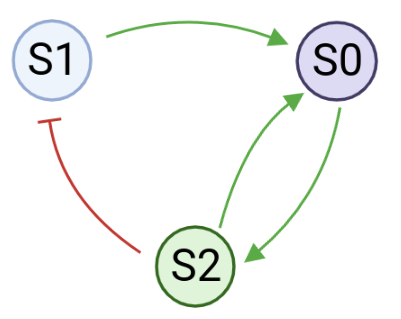
\includegraphics[width=5cm]{images/feedback-cycle.png}
    \captionof{figure}{Species interactions of Network B. Green arrows indicate activation and blunt red arrows indicate inhibition. The interactions form a cycle with negative feedback suggesting that Network B is a feedback oscillator.}
    \label{fig:feedback}
\end{center}


\section{Discussion}

Oscillating models were significantly enriched for autocatalytic reactions compared to control networks. Most oscillators are associated with unstable steady states. Destabilizing processes can be classified as 1) direct autocatalysis, 2) indirect autocatalysis (a positive feedback loop), and 3) end-product inhibition (a negative feedback loop)~\cite{Tyson1975, tyson2007}. Reactions are considered autocatalytic when the products increase the rate of reaction or when a chemical decelerates the rate of its own destruction~\cite{Tyson2004}. Given the two types of oscillators, negative feedback and negative feedback coupled with positive feedback~\cite{Sauro_dynamics}, it is unsurprising that autocatalytic reactions are enriched in the oscillator population as these reactions are a form of positive feedback. The portion of models containing at least one autocatalytic reaction in the oscillator and control populations were compared using a two-way chi square test. Of the 586 oscillating models, 83.1\% (487 of 586) contained an autocatalytic reaction compared with 49.8\% (498 of 1000) of the control models, a significant difference ($p < 0.0001$). 

Given the enrichment of autocatalytic reactions, one might expect a similar enrichment of degradation reactions, reactions where one species is removed from the system (eg. $X + Y \to Y$, where $X$ is removed from the system), to prevent species concentrations from rising to infinity. Interestingly, the presence of degradation reactions were not enriched in oscillating models. Of the oscillating model population 79.4\% (465 of 586) contained at least one degradation reaction compared to 76.3\% (763 of 1000) of the control models, an insignificant difference suggesting that although autocatalysis is a common characteristic in oscillating networks, degradation reactions are not necessary to prevent species concentrations from rising to infinity.  Although the presence of both an autocatalytic and a degradation reaction are not necessary for oscillation, it is rare that an oscillator contains neither. Only 0.5\% (3 of 586) of the oscillators analyzed had neither an autocatalytic reaction nor a degradation reaction compared to 0.2\% (2 of 1000) random models, an insignificant difference.

To determine if any reaction types were enriched in the oscillator population compared to the control population, the average model compositions were compared. The average model composition was assessed as the average number of reactions of the specific type were divided by the average total number of reactions for each group. For example, there were an average of 6.592 reactions per model in the oscillator population, of which an average of 0.99 were uni-uni reactions, for an average of 15.3\% uni-uni reactions in the average oscillator model (Table \ref{fig:avg-comp}). Compositions were compared with permutation tests, showing that model compositions and sizes were significantly different between the oscillator and control populations (the reduced size of oscillating networks can be accounted for by the fusion of duplicate reactions). Oscillators possessed significantly more uni-bi reactions compared to random control models. This is consistent with the enrichment of autocatalytic reactions which are often uni-bi. However, autocatalytic reactions can also be bi-bi reactions, which were not enriched in oscillating models. Although bi-bi reactions were less likely to be created during evolution due to the initial settings (10\%), it is somewhat surprising that bi-bi reactions were decreased in oscillatory networks given that a bi-bi reaction is slightly more likely to be autocatalytic ($\frac{4}{27}$) compared to a uni-bi reaction ($\frac{1}{9}$).

\begin{center}
    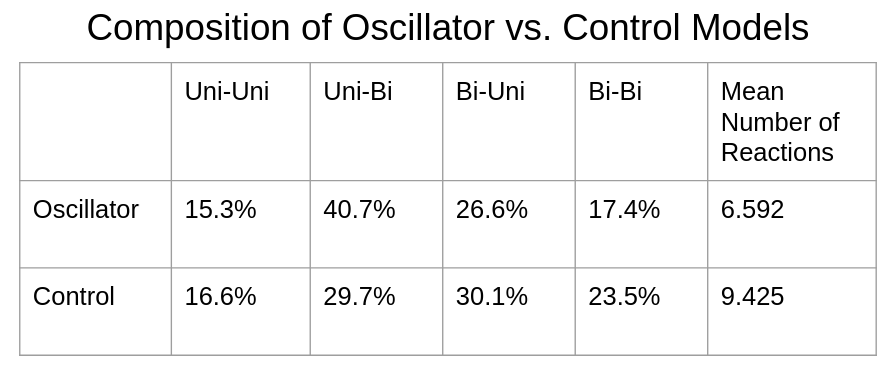
\includegraphics[width=8cm]{images/composition.png}
    \captionof{table}{Average reaction compositions of oscillating networks compared to non-oscillating controls.}
    \label{fig:avg-comp}
\end{center}

Next, oscillators containing autocatalytic reactions (498 models) were compared to oscillators lacking them (98 models). Populations were compared by permutation test. There was a significant increase in the portion of uni-bi reactions and a significant decrease in the portion of bi-uni reactions in non-autocatalytic models as compared to autocatalytic oscillators (Table \ref{fig:autocatal}). This result is interesting given that autocatalytic reactions are either uni-bi or bi-bi and both reaction types were reduced in oscillators with autocatalytic reactions compared to oscillators without. It is possible that oscillators without a single autocatalytic reaction are achieving autocatalysis through a combination of non-autocatalytic reactions.

\begin{center}
    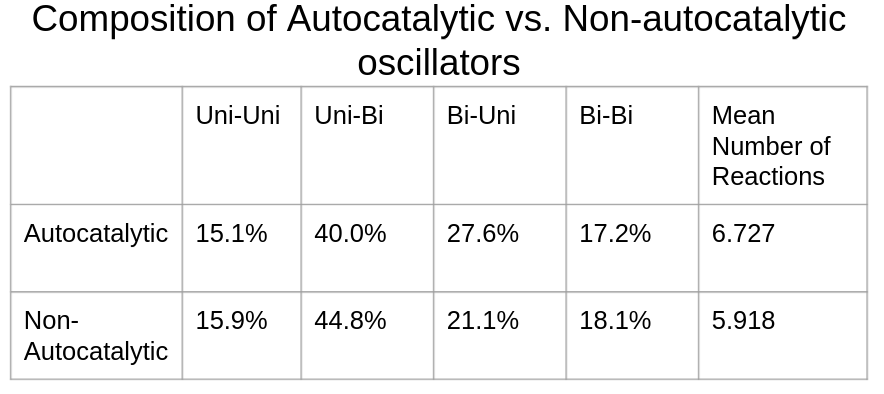
\includegraphics[width=8cm]{images/autocomp.png}
    \captionof{table}{Average reaction compositions of autocatalytic oscillating networks compared to non-autocatalytic oscillating networks.}
    \label{fig:autocatal}
\end{center}

Several manually inspected oscillators had reactions with extremely high rate constants (greater than 300, whereas most rate constants were between 5 and 75). The initial range for rate constants is 0 to 50 and with each mutation, they can only increase a maximum of 15\% of the current value. Although there is no upper limit for rate constants, it is nearly impossible to mutate a rate constant from the initial range to over 100 during the course of evolution. To bypass this limit and achieve high rate constants, many successful models have simply duplicated reactions during the evolutionary process. During post-processing, these duplicate reactions are fused and their rate constants summed. Fusing duplicate reactions to achieve high rate constants accounts for the observation that oscillators generally have fewer reactions than non-oscillators in this study. These high rate constant reactions can not be removed, nor can the rate constant be significantly lowered without impacting oscillation. Further investigation is needed to determine what essential function these high rate reactions seem to play in most of the oscillators included in this study. 


These oscillatory models and the random control networks have been added to a database, accessible at \url{https://cesiumdb.herokuapp.com/}. Models can easily be selected by the number of species, the number of reactions, and the present of autocatalysis or degradation reactions. The selected models can be downloaded in a zip file containing a .txt for each model. Each .txt file contains an individual model's antimony string. If the "Download in simulatable Tellurium form" option is selected, the .txt file will also contain formatting and package imports allowing the model to be easily simulated when the file is run as a python script. 

In the future, this database will be expanded to contain a variety of models with different behaviors besides oscillation. It is our hope that this database serves as a resource for the modeling community to study network behaviors and test novel software.


\section*{Funding}
This project was supported by National Institute of Health grant U01 CA238475 and the National Institute of Biomedical Imaging and Bioengineering for grant P41GM109824.

\section*{Acknowledgements}
We thank Lucian Smith for valuable discussions on differential evolution and model topology. 
\\
\\
This chapter was adapted from the following publication:
\\
\textbf{Tatka, L.}, Luk, W., Hellerstein, Elston, T., J., Sauro, H. “Cesium: A Public Database of Evolved Oscillatory Reaction Networks.”  Biosystems, vol. 224, 2023, p.104836., \\
https://doi.org/10.1016/j.biosystems.2023.104836. 
\\

\chapter{Parking lot for abandoned text that might be useful later}
Applying GAs to problems of parameter optimization is fairly straightforward as ``chromosomes" can be sequences of values, easily mutated and crossed over with other strings of values. This approach becomes more complex when applied to network problems, where network topology is deeply intertwined with parameter values. In these problems, the challenges becomes innovating while preserving decent candidate solutions. 
At its core, NEAT employs a genetic algorithm to evolve populations of neural networks. Each individual in the population represents a neural network with its own unique topology (i.e., arrangement of nodes and connections). NEAT starts with a population of simple neural networks, often with minimal structure, and evolves them over generations to solve a given task.

One of the key innovations of NEAT is its ability to handle the complex task of evolving neural network topological structures. NEAT accomplishes this by employing three main mechanisms: speciation, historical marking, and structural innovation. Speciation encourages diversity within the population by comparing individuals against similar individuals as opposed to the entire population. This shelters innovations that may be weak at first, but will develop into robust solutions over several generations. A historical record of topological innovations serves as a "chromosome" and enables meaningful crossover without computationally expensive matching procedures required in other algorithms. Lastly, NEAT allows for the introduction of new structural innovations in neural networks through mutation. New nodes and connections can be added to existing networks, providing the potential for incremental growth and improvement over successive generations.

\section{Existing Software}

Although there are numerous studies implemting genetic algorithms in systems biology applications, few software packages exist to aid in this pursuit. In 2008, Kratz and Krishna developed GeNESis, a C based software with GUI to enable evolution of gene regulation networks. Its purpose was to help researchers undersatnd the evoltuionary behavior of populations of genetic regulatory networks. Connections were represented by binary strings, enabling the use of crossover. The URL to this tool is currently inactive.

Chandran and Sauro devloped a C library with basic functions for evolution of biological networks including genetic networks, protein networks, and mass-action networks. Although highly versatile, the library requires some C programming knowledge in order to customize the evolutionary algorithm.

\section{CRN basics}
The projects described focus on computational models of (bio)chemical reaction networks (CRNs). Although several modeling paradigms exist to describe CRNs, this work uses CRNs represented by systems of ordinary differential equations. A CRN is a set of chemical reactions $R_i$ where i is the index over the range 1 to n, the total number of reactions in the network . Reactions involve the chemical species of the network, $S_j$ where j is the index of each species from 1 to the total number of species. A reaction is then represented as follows:
\begin{equation*}
Ri: \sum_{j\in S}^{}\alpha_{ij}S_j\to \sum_{j\in S}^{}\beta_{ij}S_j
\end{equation*}
where $\alpha_{ij}$ and $\beta_{ij}$ are non-negative integers, stoichiometry coefficients. For example, a simple 3-species, 2-reaction network can be represented by the following reactions:
\begin{equation}
\begin{split}
S1 + S2 \to S3 \\
S3 \to S1 + S2
\end{split}
\end{equation}
However, these reactions alone are insufficient to completely describe the small network. The rate constants and rate laws for the reaction are unspecified. This research focuses on mass-action kinetics, where the rate of a reaction is dictated by the concentration of its substrates and a rate constant:
\begin{equation}
\begin{split}
S1 + S2 \to S3; \;\;\;\;\;\; k_1*S1*S2\\
S3 \to S1 + S2; \;\;\;\;\;\;\;\;\;\;\;\;\; k_2*S3
\end{split}
\end{equation}
The rate of change of each species can then be put in the form of a differential equation (equation 1.3) and solved numerically.
\begin{equation}
\begin{split}
\frac{dS1}{dt}=k_2S3 - k_1S1S2\\
\frac{dS2}{dt}=k_2S3 -k_1S1S2\\
\frac{dS3}{dt}=k1S1S2 - k_2S3
\end{split}
\end{equation}

\chapter{In Silico Speciated Evolution of Oscillatory Mass-Action Reaction Networks}
\label{chap: NetEvolve}
Genetic algorithms (GAs), inspired by the principles of natural selection and genetics, have emerged as a powerful computational technique for solving optimization and search problems.Developed by John Holland in the 1970s, GAs mimic the process of biological evolution to solve optimization and search problems \cite{holland_1975}. At their core, genetic algorithms operate on a population of potential solutions, represented as individuals or ``chromosomes," each encoding a candidate solution to the problem at hand. Through iterative generations, genetic algorithms apply mechanisms of selection, crossover, and mutation to evolve and refine the population, gradually converging towards optimal or near-optimal solutions. Selection favors individuals with higher fitness, mirroring the process of natural selection, while crossover and mutation introduce variation and diversity into the population, allowing for exploration of the solution space. By leveraging the principles of evolution, genetic algorithms offer a versatile and robust approach to solving complex problems across various domains, from engineering and optimization to biology and beyond.

Francois and Hakim were among the first to apply genetic algorithms to systems biology \cite{francois_hakim_2004}. In an effort to generate small genetic networks that functioned as bistable switches and oscillators, they implemented a simple genetic algorithm to evolve both the structure and rate constants of idealized abstractions of genetic regulatory networks. The  algorithm used only mutation and selection, avoiding crossover, to minimize the difference between the candidate networks' output and idealized time series data displaying the desired behavior. Although the evolutionary scheme was relatively simple, they achieved promising results which encouraged the exploration of evolutionary techniques on similar problems.

Fujimoto et al. employed a similar strategy to study genetic networks leading to striped patterning and ultimately body segmentation in arthropods \cite{fujimoto_network_2008}. When analyzing the resulting networks, they found three distinct classes, feed-forward loops, feed-back loops, and interconnections between the two. These three classes reproduced various segmentation strategies observed in arthropods.

Kobayashi et al. also explored the evolution of oscillatory genetic networks, however their algorithm fixed parameter values and only allowed connection rewiring to achieve oscillations with prescribed time periods \cite{kobayashi_evolutionary_2010}. Deckard and Sauro expanded this concept beyond genetic regulatory networks to evolve small networks with specific computational capabilities such as square root and cube route calculators \cite{deckard_preliminary_2004}. As with the previously mentioned algorithms, their algorithm avoided crossover relying solely on mutation to develop candidate solutions. Attempts to use crossover did not result in fitter offspring, possibly due to combining heterologous networks and thus disrupting developing solutions. This work was continued by Paladugu et al seeking to generate mass-action network functional modules with specific behaviors, including oscillators \cite{Paladugu2006}.  This algorithm avoided crossover as the authors argued that it would be disruptive.

Marchisio and Stelling argued that brute force optimization algorithms lack efficiency and that implementing some element of rational design could speed up automatic design of genetic networks implementing boolean logic gates \cite{marchisio_automatic_2011}. They separate structural and parameter optimization by first generating several possible circuits and then ranks feasibility based on the structure. Then the best solutions undergo parameter optimization. Separating structural design from parameter optimization certainly saves computation time, but it relies on the existence of a rational solution, and is better suited for genetic networks, where these attributes are more easily separated. For more complex tasks, a solution might depend on a precise combination of both structure and parameter.

Other approaches fix structure and make use of evolutionary algorithms to explore the parameter space while fixing network topology. Jin and Sendhoff used an evolution strategy to explore parameters of regulatory motifs with fixed structures \cite{jin_evolving_2008}. Porubsky and Sauro use an evolutionary algorithm to search for parameters that yield oscillations in mass-action networks of fixed structure \cite{porubsky2019}.


Most applications of evoltuionary algorithms in systems biology avoid the use of crossover as it tends to disrupt candidate solutions. For example, Drennan and Beer successfully evolved a repressilator (a specific type of oscillatory reaction netowrk \cite{Elowitz2000}) using a genetic algorithm that included crossover \cite{drennan_beer}. However, due to the encoding of the network graph, there was a high probability of breaking connections making it difficult to pass on structural innovations. Stanley and Miikkulainen addressed this problem in 2002 with NEAT (NeuroEvolution of Augmenting Topologies), a powerful algorithm used for evolving artificial neural networks (ANNs) \cite{stanley_evolving_2002}. Unlike traditional methods of neural network training, which typically involve adjusting the weights and biases of fixed network architectures, NEAT evolves both the structure and weights of neural networks simultaneously. A two key features of NEAT are the use of a more meaningful structural crossover technique, and speciation, which protects innovations and allows them time to develop by having candidate solutions compete only against similar individuals instead of the entire population. Dinh et al. adapted this technique to genetic regulatory networks and found improved performance in evolving oscillators with the use of crossover.

This work describes the adaptation of the NEAT algorithm to mass-action chemical reaction networks and explores the utility of crossover, speciation, and other hyper-parameters in evolving oscillatory networks. A software package to systematize the study of hyperparameters is introduced. This package, written in the julia programming language \cite{bezanson2017julia}, simplifies the customization of evolutionary algorithms. It has broad applications as it can be run from the command line and allows users to specify settings in a json file. It is capable of matching any time series data. 


\section{Evolving Reaction Networks}
The purpose of this work it twofold: (1) to create a general purpose, easily customizable, module for evolving mass-action chemical reaction networks and (2) to explore the effects of crossover,  speciation, and other hyperparameters on the success rate of the algorithm. Oscillatory chemical reaction networks were chosen as the target result of the evolutionary algorithm due to their biological relevance, poorly understood architectures (maybe??), and the presence of intermediary states (damped oscillations) which aids in gradual evolution.
----

Oscillatory behavior is useful in a variety of biological processes including p53, circadian rhythm, and cell cycle. But also, you might want to generate oscillators as a component in a syntehtic biology ciruit. But really, this isn't about oscillators, that's just the test case. You might want a certain behavior and don't know how to build a  network to get it. Well This algorithm is for you! 

Other people have done similar things, but this is different. It starts with the concept of genetic algorithms, way back in 1975. These are algorithms to come up with optimization solutions. The algorithms kind of look like biologic evolution. You have a bunch of individuals, the fitter individuals share their genes and reproduce, less fit individuals die off, sometimes mutations occur and these can be either good or bad. Since then, the concept of genetic algorithms has been thoroughly explored, but here we present something slightly new. And that's how I'm going to get my PhD lol.

This all starts with the NEAt algorithm which is a way of evolving neural networks to do stuff.  What's interesting about this is they claim to have meaningful crossover and they use speciation to protect innovation. Dinh et al somehwat adapted this appraoch to genetic circuits, but those are a much easier problem because they just have activation and inhibition. Here, I adapt this algorthim to mass-action networks. That's way harder because there is way more complexity. In the first case, you just have an edge that connects two nodes and a weight. In the second, you add that the edge can either be activating or inhibiting, but here we add that the edge could connect multiple nodes (in the case of everything beyond a uni-uni reaction) and the reaction weight depends on what nodes it connects. More on that later.

I need to go over a bunch of times that this was done for a similar thing. Just as a quick review


---------------------------------
Some review stuff


Evolutionary design of oscillatory genetic networks (Kobayashi 2010)
Wanted to evolve genetic oscillatory networks. Get a large population of them and then mine them for statistics about oscillators and network motifs. They have fixed parameter values though and only change connections (?). Looks like they are also trying to evolve oscillators with specific frequencies. They have a cost function which looks at periodicity




\section{Methods}

\begin{center}
    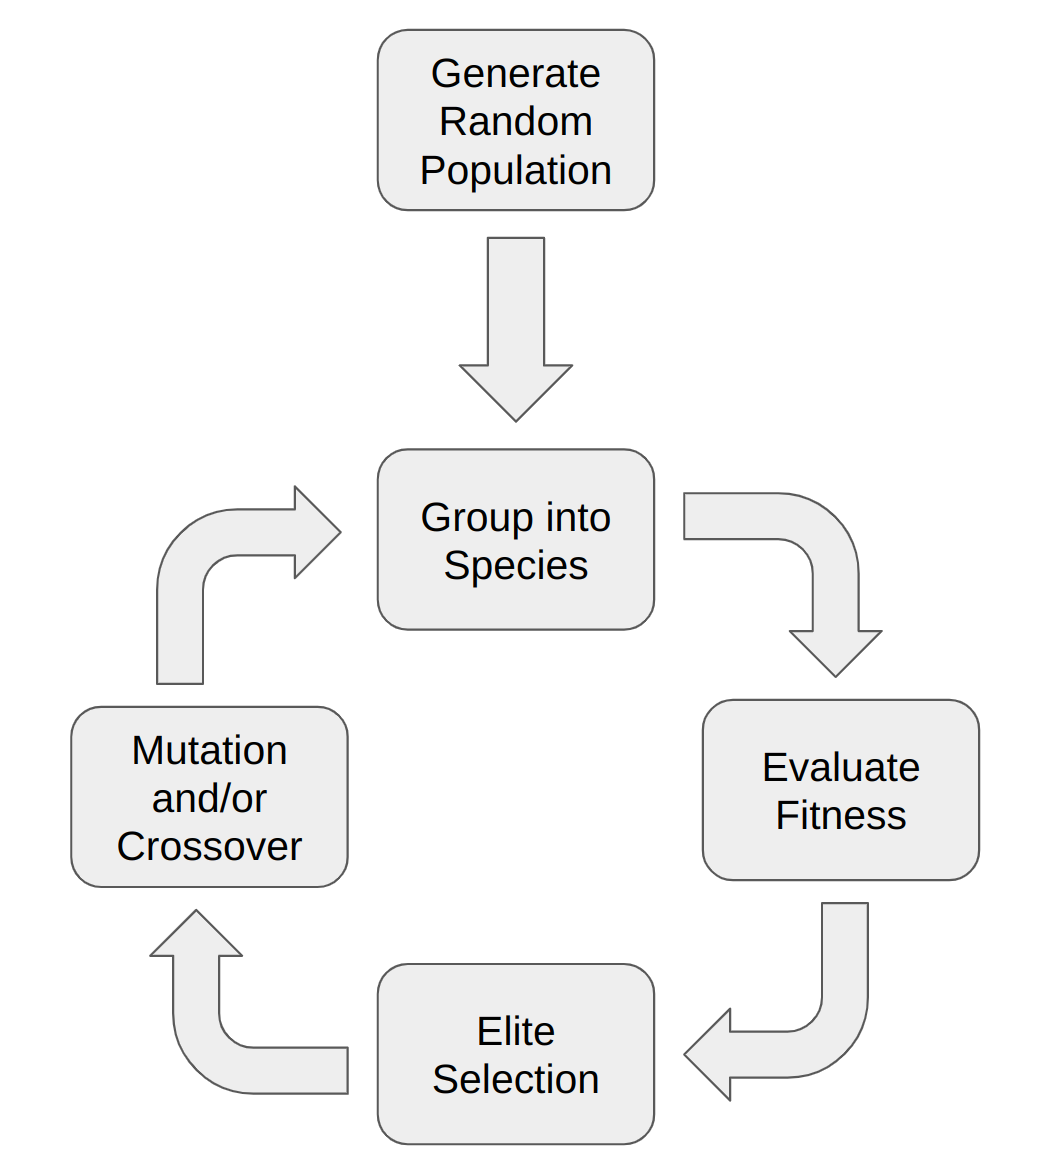
\includegraphics[width=8cm]{images/algo_description_crossover.png}
    \captionof{figure}{The evolutionary algorithm begins with a population of randomly generated reaction networks. These networks are then grouped into species and their fitness evaluated. The next generation is constructed by first selecting the top performing individuals from each species without modification. The rest of the subsequent generation is populated by networks that are modified by either crossover, mutation, or both. This new generation is then grouped into species based on structural similarity and the process repeats.}
    \label{fig:algo_description_crossover}
\end{center}
\subsection{Encoding}
Chemical reactions are represented as custom data structures that contain one or two reactants, one or two products, a rate constant, and a boolean value indicating if the reaction is active or inactive. Four types of mass-action reaction are possible: uni-uni (a single reactant to a single product), bi-uni (two reactants form a single product), uni-bi, and bi-bi. A reaction that is active participates in the network that it is part of. An inactive reaction is ``turned off" but remains part of the network as a historical record. It can be activated again or crossed over under certain circumstances. 

A reaction network is a custom data structure consisting of several reactions, initial concentrations for the floating species, and other information to track the individual network. A network can include boundary species (which are assumed to be at a constant concentration throughout the simulation), but boundary species were not used in this study.

\subsection{Mutation}
\label{section: mutation}
There are two types of mutation: rate constant mutation and reaction addition or subtraction. The probability of each of these mutations occurring and the range in which rate constants are mutated can be set by the user. A rate constant mutation can occur in two possible forms. The rate can be increased or reduce by a random percentage, uniformly distributed in a custom range (by default $\pm20\%$), or more rarely a completely new rate constant can be selected, uniformly distributed within a custom range (by default 0.1 to 50). Rate constants were not allowed to become negative, but they did not have an upper bound as previous studies observed that many synthetic oscillating systems rely on a single reaction with an abnormally large rate constant \cite{Tatka2023}.

A reaction mutation is either the addition of a new random reaction or the deletion of an existing reaction, with 50\% chance of each. When a new reaction is added, it is generated randomly with a 
probability of 0.1, 0.4, 0.4, 0.1 for uni-uni, uni-bi, bi-uni, and bi-bi reactions respectively. These probabilities are also configurable. If the randomly generated reaction is already present in the reaction network, the new reaction's rate constant is added to the existing reaction's rate constant. This feature can allow some rate constants to grow to several multiples of the next largest rate constant in the network. When a reaction is deleted, it is ``switched off" and becomes inactive in the network, but is preserved as it can become reactivated under certain circumstances.

\subsection{Crossover}
During crossover, two parent networks from the same species group are chosen to mate. If a reaction is present in both parents, the reaction will be passed down to the offspring network with the rate constant randomly chosen from one parent. If a reaction is present in the more fit parent, but not the less fit parent, the offspring network will inherit the reaction. If an inherited reaction is currently inactive meaning it was previously deleted during a mutation step), there is a 0.25 probability of the reaction becoming active again. If both parents are equally fit, one is randomly chosen to be the more fit parent. 

\subsection{Speciation}
In many cases, modifying a network, especially through the addition or deletion of reactions, initially makes the system less fit. Without speciation, these innovations seldom last for more than a generation. However, often these topological innovations prove an essential step in evolution \cite{stanley_evolving_2002}. For this reason, a speciation strategy is employed to protect innovations and allow them time to optimize. Individuals with similar topologies are grouped into species. Members of a species compete only with each other and not the population at large.  A compatibility distance metric, $\delta$, is used to assign reaction networks to a species, defined as

\begin{equation}
\delta=\frac{M}{N}
\end{equation}
where M is the number of reactions in the larger network that are not present in the smaller network and N is the total number of reactions in the larger network. Two reactions are considered identical if they have the same reactants and products. Rate constants are not considered. If $\delta$ is below the speciation threshold, $\delta_{t}$, the two networks are members of the same species.

For each new generation, networks are assigned to species based on the previous generation's species groups. Each new network is compared to a randomly chosen individual from a species in the previous generation. If $\delta$ is less than the speciation threshold $\delta_{t}$, then the network is assigned to that species. If $\delta$ is greater than $\delta_{t}$, then the network is compared to a randomly selected individual from the next species, etc., until a match is found. If no species is assigned after comparing the network to all species in the previous generation, then a new species is created. 

The speciation threshold $\delta_{t}$ is adjusted with each generation to steer the total number of species towards the target number of species. The target number of species is 10 by default, but can be configured by the user. After each generation the total number of species is counted. If there are more species than the target value, $\delta_{t}$ is increased allowing networks that are more dissimilar to be grouped together. If there are fewer species than the target value, $\delta_{t}$ is decreased. Adapting $\delta_{t}$ as evolution proceeds maintains an optimal number of species. If there are too many species each with a small number of members, there are not enough opportunities to optimize solutions in a small parameter space. Similarly, if there are too few species with several members, the entire parameter space is not adequately explored. 

\begin{equation}
	\delta_{t} = \begin{cases}\delta+\epsilon,& \mbox{if number of species} > N_{s} \\
	\delta-\epsilon,& \mbox{if number of species} < N_{s}
	\end{cases}
\end{equation}

\subsection{Objective Function}

The objective function evaluated how well a candidate model oscillated at the imposed time period, $T$.  Two arbitrary concentrations, $[C]_{1}$ and $[C]_{2}$,  were chosen \textit{a priori}. The fitness score of a particular network was then attributes to how well any of its chemical species approached $[C]_{1}$ at half periods ($T/2$, $3T/2$, $5T/2$,...) and  $[C]_{2}$ at each period ($T$, $2T$, $3T$,...) over the course of 5.5 periods. The candidate model's single chemical species that best approached these points was selected and the fitness was evaluated as the maximum of the reciprocal of the absolute difference between the timeseries data and $[C]_{1}$ or $[C]_{2}$, the ``ideal oscillator" time points, (equation \ref{equation: fitness}). The reciprocal was taken so that higher values represented better fitness, which is necessary for determining the number of offspring for each species in subsequent steps. This objective function has been shown to be an effective means of evolving oscillators in similar and previous works \cite{Paladugu2006, francois_hakim_2004, Tatka2023}. In cases where candidate models could not be simulated, a fitness of 0.0 was assigned resulting in the candidate model's subsequent removal from the population.

\begin{equation}
\label{equation: fitness}
fitness = max(\frac{1}{\sum|ideal - candidate|})
\end{equation}

\subsection{ODE Solver}
During the fitness evaluation phase, reaction networks were converted to systems of ordinary differential equations. These equations were then numerically solved using the DifferentialEquations.jl julia package \cite{DifferentialEquations.jl-2017} and the CVODE solver from the Sundials suite for solving initial value problems \cite{hindmarsh2005sundials}. The CVODE solver was shown to be effective for this application in previous work \cite{Tatka2023}.

\subsection{Reproduction}
Each model species was allotted offspring in proportion with its fitness. More fit species were allowed more offspring. To calculate the number of offspring allotted to each species group the sum of fitness values was computed across the entire population. Then each species, $s$, was assigned an offspring number proportional to its contribution to the fitness of the entire population (equation \ref{equation: num_offspring}). The calculated number of offspring for each species was rounded to the nearest integer. By default, a single species was only allowed to produce at most 10\% of the subsequent generation in order to prevent a single species from taking over the entire population (but this value could be adjusted by the user). For these reasons, the total number of individuals fluctuated slightly over time.


\begin{equation}
\label{equation: num_offspring}
offspring_{s} = \frac{\sum{fitness_{s}}}{\sum{fitness_{pop}}}*populationsize
\end{equation} 

The reproduction phase began with an elitism selection strategy. The top 10\% of networks in each species were copied to the next generation directly. If a species had 10 or fewer individuals, the single best network was copied without modification to the next generation. Then, the bottom 10\% of networks in each species are deleted. For the remainder of the allotted offspring for each species, a random number, $p$, was generated. If the $p$ was less than the probability of crossover, then two networks from the same species were selected and crossed over to produce a single offspring network. Otherwise a single network was chosen. If $p$ was greater than or equal to 1 - the probability of mutation, the network was mutated. Outside of the elite networks, all networks were either crossed over or mutated. Some were both crossed over and mutated. The probabilities of crossover and mutation could be configured by the user. Probabilities for specific types of mutations are described in section \ref{section: mutation}.

Tournament selection was also explored and can be configured in settings. In this case, two networks from the same species were randomly chosen and the more fit network was then crossed over, mutated, or both. If crossed over, a second network was also chosen by tournament selection.

\subsection{Output}
The evolutonary aglorithm was repeated for a preset number of generations (800 by defualt) or until the best model reached a predefined fitness level. At this point, the best model from each species was converted to Antimony, a human readable model definition language \cite{Smith2009} and written to a text file along with the model's fitness. All settings were also written out to a JSON file, which could be used without modification to repeat the evolution trial.

The best models from each evolution trial were automatically assessed with a Python script using the Tellurium modeling environment \cite{Choi2018} and RoadRunner simulation software \cite{andy2020}. A model was considered an oscillator if its Eigen values at steady state contained a positive real number with a nonzero imaginary number and if all concentrations were positive at steady state. Models that met the Eigen value criteria but had negative steady state concentrations were flagged. Flagged models then underwent a simple automated repair process wherein each reaction was deleted one at a time in an effort to meet the oscillation criteria. Models that met criteria after the simple repair process were counted as oscillators.

\section{Results}
The software was evaluated with multiple hyperparameter settings to assess its ability to generate oscillatory mass-action chemical reaction networks. Each set of hyperparameters were evaluated over 700 evolutionary trials and the success rate recorded. A trial was deemed successful if it generated a network with sustained oscillations, as evaluated by the criteria described previously.

\subsection{Speciation Maintains Diversity and Increases Success Rate}
\label{section:speciation}
In order to test the effects of speciation on population diversity and oscillator success rate, evolution was run without speciation, and with 10 and 30 as the target number of species. When speciation is disabled, the top 10\% of the entire population is passed on to the next generation unmodified and the bottom 10\% of the entire population is deleted. Then mutation is performed on the entire population to populate the remainder of the subsequent generation (crossover was not performed for these experiments). Each network must compete against every other network in the population. To account for fluctuations in population size when speciation is enabled, diversity was measured as the number of unique networks over the total number of networks in the population. A network was considered unique if differed by one or more reactions from all other networks. Reactions are considered different if they differ in product or reactant. Rate constants are not considered in these comparisons. Significance levels were calculated using two-tailed t-tests. 

In trials where no speciation was allowed, the average portion of unique networks was 0.228 $\pm$ 0.026 across 800 generations. This is significantly (p \textless 0.0001) less than the portion of unique networks in evolution trials with a target number of species of 10, 0.298 $\pm$ 0.033 (figure \ref{fig:num_unique_species}).

\begin{center}
    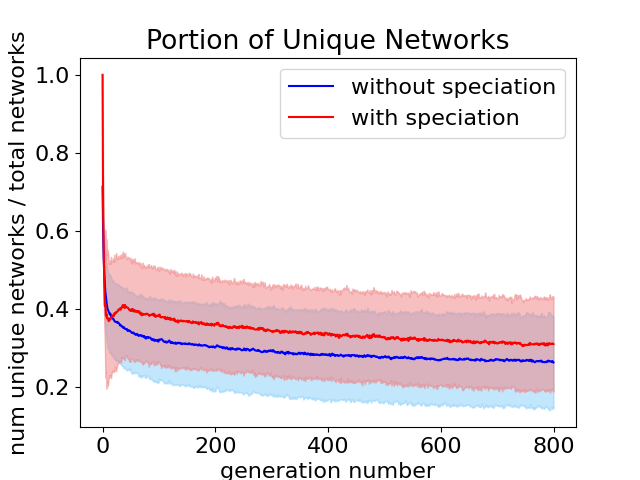
\includegraphics[width=18cm]{images/num_unique_networks.png}
    \captionof{figure}{The average portion of unique networks over 800 generations with speciation (left), 0.0298 $\pm$ 0.033, and without (right), 0.228 $\pm$ 0.026. Dark blue line represents the average portion for each generation and light blue shading is the 95\% confidence interval.}
    \label{fig:num_unique_species}
\end{center}

One purpose of speciation was to prevent the most fit network from overtaking the population over time. When a single network dominates the population, there are not enough unique networks to adequately explore the solution space and the evolution algorithm converges on a solution prematurely. To account for fluctuating population sizes when speciation is allowed, the number of copies of the best network divided by the total number of networks was measured at each generation with speciation (with a target species number of 10) and without speciation.  When speciated was enabled, the portion of the population occupied by copies of the most fit network remained constant with an average portion of best networks of 0.079 $\pm$ 0.011. Without speciation, the portion of best networks rose gradually over time with an average portion of 0.495 $\pm$ 0.094 (figure \ref{fig:portion_best_network}). This shows that speciation effectively prevents a single network from dominating the population (p \textless 0.0001).

\begin{center}
    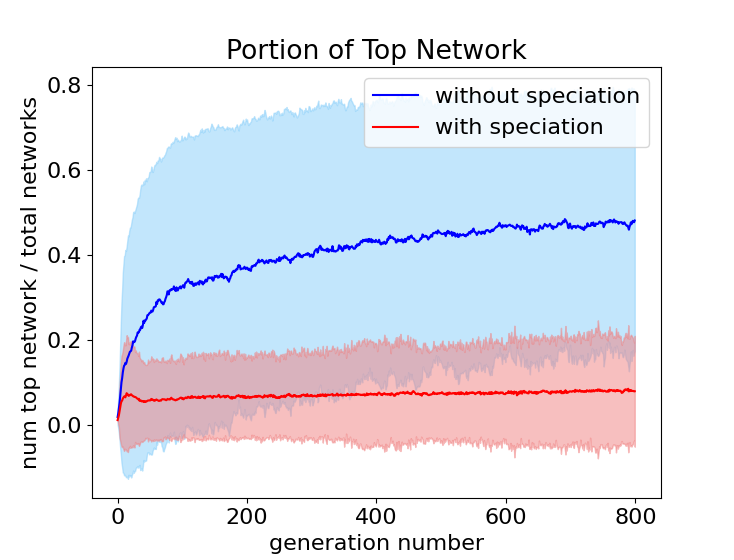
\includegraphics[width=18cm]{images/portion_best_network.png}
    \captionof{figure}{The average portion of best networks over 800 generations with speciation (left), 0.079 $\pm$ 0.011, and without (right), 0.495 $\pm$ 0.094. Dark blue line represents the average portion for each generation and light blue shading is the 95\% confidence interval.}
    \label{fig:portion_best_network}
\end{center}


Next, the effects of speciation on evolution success rate was evaluated comparing no speciation to speciation with a target species number of 10 and 30. Again, crossover was omitted from these studies. For each speciation level, a batch of 700 trials of evolution were run and the number of oscillators resulting from each batch. Significance levels were calculated using a binomial distribution. 

With a target species of 10 (the default condition), evolution trials resulted in sustained oscillators at a rate of 0.19 (134/700). Without speciation, the success was significantly reduced (p \textless 0.0001), with oscillators occurring at a rate of 0.06 (44/700). TO more thoroughly evaluate the benefits of speciation, a batch of 700 evolution trials was run with a target species number of 30. This resulted in a success rate of 0.17 (117/700). This rate is not significantly different (p = 0.1127) than the rate with a target species number of 10. Speciation increases the success rate of evolution, but grouping networks into more species with fewer members does not improve success (figure \ref{fig:species_success_rate}). 

\textbf{Might be interesting to try with 50 species and see if I can get it to be worse just to make a point}
 
\begin{center}
    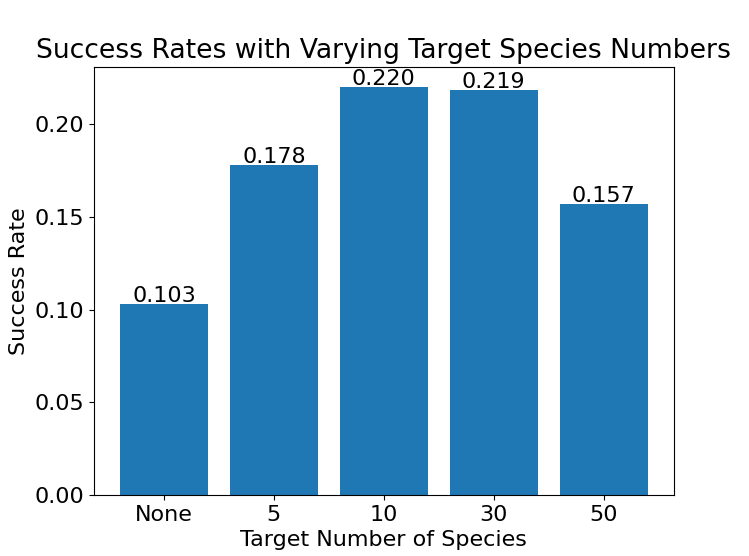
\includegraphics[width=15cm]{images/species_success_rate.png}
    \captionof{figure}{Evolution success rate of 700 trials with no speciation, with a target species of 10, and with a target species of 30. Speciation significantly improves success rate, but more species does not improve success.}
    \label{fig:species_success_rate}
\end{center}

\subsection{Crossover Does Not Improve Success Rate}
Batches of 700 evolution trials with and without crossover were compared. The batch without crossover was the same batch described in \ref{section:speciation} with a target species number of 10 and a success rate of 0.19. This batch had 0.0 probability of crossover and 0.75 probability of mutation. This meant that there was a 25\% chance that a network was passed on to the next generation without modification. The batch with crossover used the crossover procedure described in the Methods section. The probability of crossover was 0.75 and the probability of mutation was 0.75. All networks were either crossed over or mutated ($p_{crossover} + p_{mutation} - p_{crossover} \cap p_{mutation} = 1$). This meant that networks had a 50\% chance of being crossed over and then mutated ($p_{crossover} \cap p_{mutation} = p_{crossover} + p_{mutation} -1$). With these settings, evolution trials with crossover enabled resulted in a sustained oscillator at a rate of 0.16 (112/700). This was significantly lower than the success rate without crossover (p = 0.0344).


\textbf{Just realized that in the non crossover batch, there were some networks that wouldn't get changed at all under the right circumstances. Should redo this}

\subsection{Effect of Selection Method}

\section{Discussion}
Configurability is cool. 
You could also use this to match timeseries data or evolve other network behaviors
As of today's results, it seems that people were right and there's not really a good computationally efficient way to crossover networks without wrecking them.

\section{Conclusion}
Yay I did it.

	


\begin{figure}
    \centering
    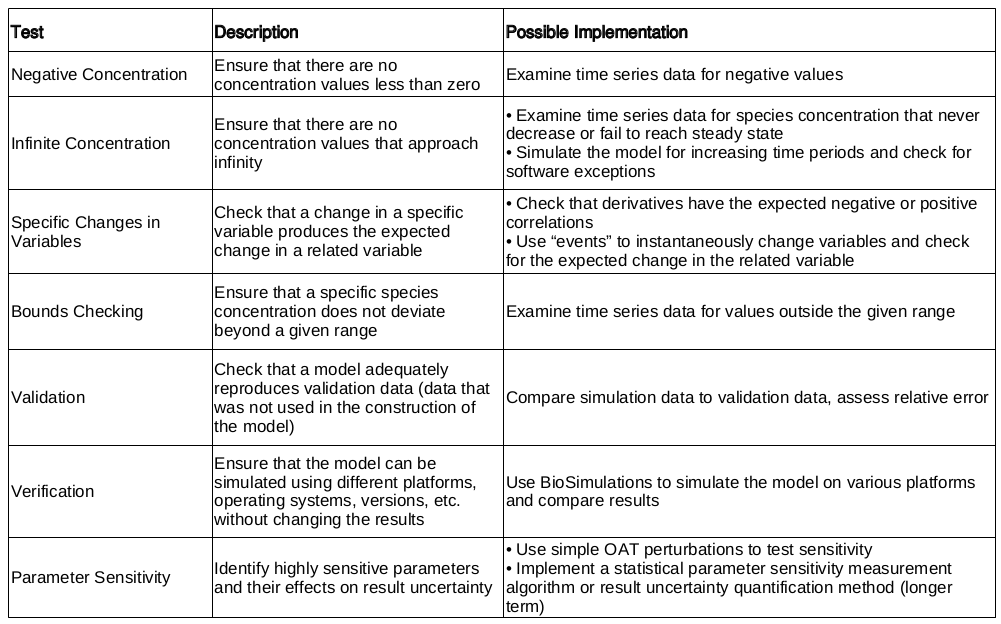
\includegraphics[width=19cm]{images/testSummary.png}
    \captionof{table}{Summary of proposed tests and possible implementations.}
    \label{table:sensitivity}
\end{figure}



% Bibliography
\bibliographystyle{unsrt}
\bibliography{researchbib}
\end{document}


